\subsection{Ca sử dụng tìm kiếm hình ảnh}

\vspace{0.5cm}

\noindent 
\begin{tabularx}{\linewidth}{| l | X |} 
\hline 
\textbf{Mô tả} & Người dùng tìm kiếm ảnh với những option hệ thống cung cấp. \\
\hline 
\textbf{Luồng cơ bản} & 1. Người dùng bấm vào nút tìm kiếm ở thanh công cụ dưới màn hình. \newline
                       2. Hệ thống điều hướng đến trang tìm kiếm. \newline
                       3. Hệ thống hiển thị các gợi ý về bộ lọc tìm kiếm (thời gian, albums, tên khuôn mặt, tên ảnh, địa điểm, truy vấn AI) và lịch sử tìm kiếm. \newline
                       4. Người dùng gõ từ khóa muốn tìm kiếm. \newline
                       5. Hệ thống hiển thị các gợi ý về bộ lọc có liên quan đến từ khóa tìm kiếm (thời gian, albums, tên khuôn mặt, tên ảnh, địa điểm, truy vấn AI). \newline
                       6. Người dùng chọn gợi ý tìm kiếm khớp với từ khóa muốn tìm. \newline
                       7. Hệ thống lưu lịch sử tìm kiếm và hiển thị kết quả theo dạng danh sách. \\
\hline
\textbf{Luồng thay thế} & - Người dùng tìm kiếm bằng giọng nói thay vì gõ từ khóa. \newline
                           - Người dùng không gõ từ khóa mà chọn gợi ý tìm kiếm. \\
\hline
\textbf{Tiền điều kiện} & - Người dùng đã đăng nhập vào hệ thống. \newline
                          - Có ít nhất 1 bức ảnh đã tải lên trong thư viện. \\
\hline
\textbf{Hậu điều kiện} & - Người dùng có thể xem thêm thông tin chi tiết về ảnh đã tìm kiếm. \newline
                          - Người dùng có thể xóa bộ lọc tìm kiếm. \\
\hline 
\textbf{Yêu cầu phi chức năng} & - Hệ thống lấy truy vấn ảnh không quá 2s. \newline
                            - Hệ thống hiển thị gợi ý tìm kiếm không quá 1s. \\
\hline 
\end{tabularx}

\vspace{0.8cm}

\noindent 
\begin{tabular}{| c | c |}
    \hline
    \textbf{Biểu đồ hoạt động} & \textbf{Quan hệ} \\ 
    \hline
    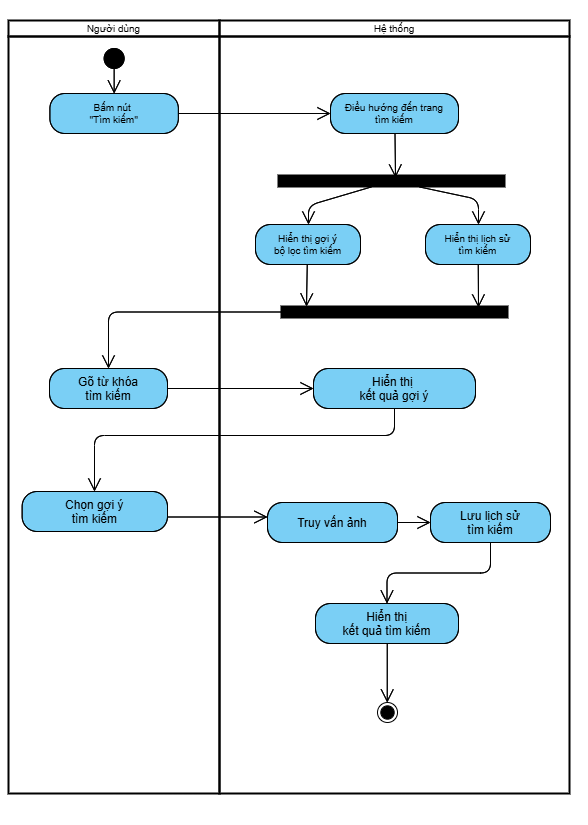
\includegraphics[width=0.6\linewidth]{figures/c3/3-3-16-activity-diagram.png} 
    &  
    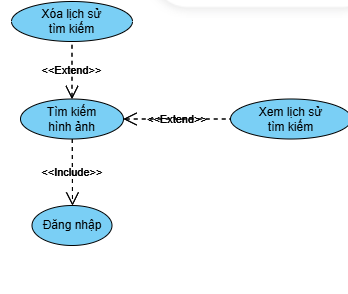
\includegraphics[width=0.35\linewidth]{figures/c3/3-3-16-relationship.png} \\ 
    \hline
\end{tabular}

\begin{figure}[H]
    \centering  
    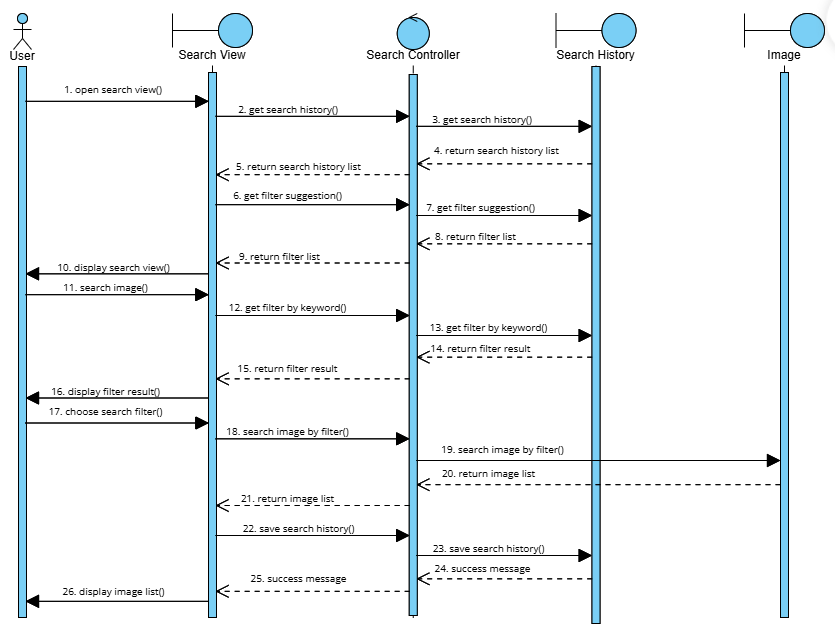
\includegraphics[width=1\textwidth]{figures/c3/3-3-16-sequence-diagram.png}
    \caption{Biểu đồ tuần tự ca sử dụng tìm kiếm hình ảnh.}
    \label{fig:3-3-16-sequence-diagram}
\end{figure}